\section{Hardware dell'adapter board}
L'hardware utilizzato per condurre lo studio oggetto di questa tesi consiste in due piattaforme indossabili per effettuare misure fotopletismografiche. Ciascuna piattaforma si compone di una Adapter Board e una scheda ospitante un microcontrollore. L'Adapter Board consiste in una PCB sulla quale sono montati il modulo PPG, un accelerometro ed un eventuale LDO per l'alimentazione dei componenti. Il microcontrollore viene utilizzato per l'acquisizione dei dati dai sensori e per il loro controllo. In particolare è stata utilizzata in entrame le soluzioni la board \textbf{STM32F4DISCOVERY}, prodotta da STMicroelectronics che ospita il microntrollore \textbf{STM32F407}. Grazie poi ad un'interfaccia USB è possibile trasmettere i dati ad un computer per permetterne l'elaborazione e la memorizzazione.
La due piattaforme progettate si differenziano per l'Adapter Board, dal momento che sono stati utilizzati due differenti moduli PPG: il \textbf{MAXM86161} e il \textbf{MAX86916}. Entrambi i sensori sono prodotti da Maxim Integrated.
\subsection{Adapter Board: MAXM86161}
\begin{figure}[b]
	\centering
	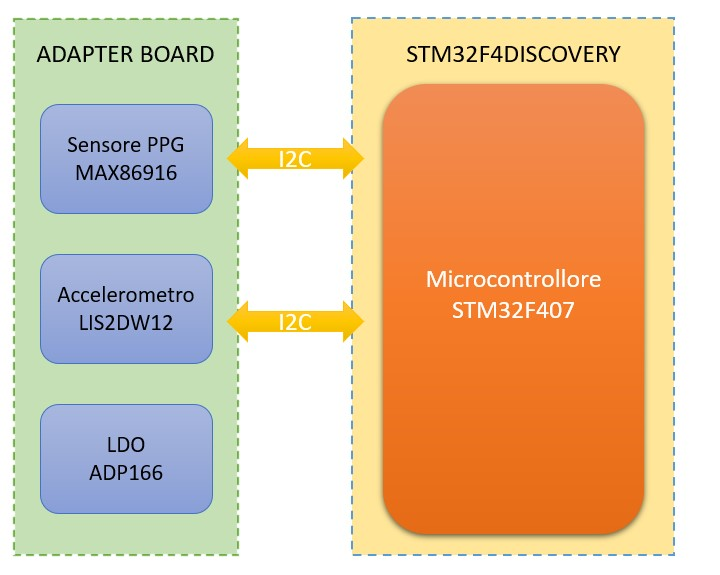
\includegraphics[width=0.6\linewidth]{ImageFiles/Hardware/DiagrammaBlocchiMAXM86161}
	\caption{Diagramma a bloccchi dell'Adapter Board}
	\label{fig:DiagrammaBlocchiMAXM86161}
\end{figure}
L'Adapter Board progettata ospita il sensore PPG MAXM96161 e l'accelerometro triassiale LIS2DW12, che comunicano con il microcontrollore tramite protocollo I\ap{2}C (\Fig~\ref{fig:DiagrammaBlocchiMAXM86161}). Grazie al numero ridotto di componenti è stato possibile ottenere una scheda dalle dimensioni molto ridotte (12,4 mm x 4,6 mm).

\paragraph{Sensore PPG} Il sensore PPG utilizzato è il MAXM86161 rappresentato nella figura \ref{fig:ImmagineMAXM86161}.
\begin{figure}[tb]
	\centering
	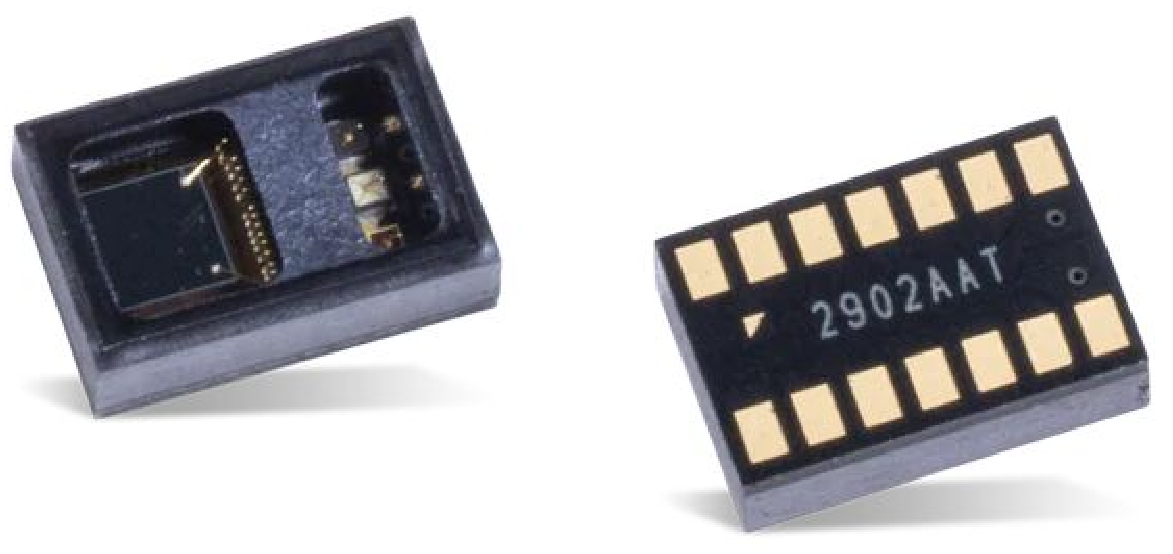
\includegraphics[width=0.8\linewidth]{ImageFiles/Hardware/ImmagineMAXM86161}
	\caption{Il modulo MAXM86161.}
	\label{fig:ImmagineMAXM86161}
\end{figure}
Si tratta di un modulo integrato a basso consumo, per acquisizioni di dati ottici. Il sensore integra 3 LED (rosso, infrarosse e verde), un fotodiodo ed elementi ottici. All'interno è anche presente un regolatore di tensione lineare (LDO). Per questo motivo non è necessario inserire un ulteriore LDO esterno per l'alimentazione dei circuiti interni e dei LED. Per questo motivo il modulo necessita di una singola tensione di alimentazione che deve essere compresa tra i 3.0V e 5.5V. \`E presente un pin di uscita (VLDO) collegato all'uscita del regolatore interno che fornisce una tensione di 1.8V. Essa può essere utilizzata per alimentare eventuali dispositivi esterni. La comunicazione con il microcontrollore avviene grazie ai pin SDA e SCL, tipici della comunicazione I\ap{2}C. \`E stato progettato per effettuare misure intra-auricolari del battito cardiaco e di ossigenazione del sangue. Infatti, generalmente le cuffie hanno dimensioni molto ridotte e possiedono batterie molto piccole. Per questo motivo, il modulo presenta un package di tipo OLGA a 14 pin, con dimensioni 2.9 mm x 4.3 mm x 1.4 mm e il consumo è minore di \SI{30}{\micro\watt}.
\todo{dobbiamo dire che altre caratteristiche sono state descritte nello stato dell'arte?}

\paragraph{Accelerometro} Il LIS2DW12 è un accelerometro triassiale lineare realizzato con tecnologia MEMS ad alte performance e basso consumo, prodotto da STElectronics\cite{STElectronicsLIS2DW12}. 
\begin{figure}[b]
	\centering
	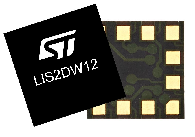
\includegraphics[width=0.3\linewidth]{ImageFiles/Hardware/ImmagineLIS2DW12}
	\caption{Accelerometro LIS2DW12.}
	\label{fig:ImmagineLIS2DW12}
\end{figure}
\`E pensato per rivelazioni di movimento e riconoscimento dei gesti su dispositivi indossabili. Il sensore permette di selezionare un fondo scala di $\pm$\SI{2}{\gram}, $\pm$\SI{4}{\gram}, $\pm$\SI{8}{\gram} oppure $\pm$\SI{16}{\gram}. Necessita un'alimentazione compresa tra i 1.62V e i 3.6V e la corrente assorbita tipicamente è di \SI{50}{\nano\ampere} nella modalità \textit{power-down} e di \SI{1}{\micro\ampere} nella modalità attiva \textit{low-power}. Inoltre, l'accelerometro include un sensore di temperatura che permette di compensare gli effetti della temperatura ambientale sulle misure. Presenta un'interfaccia I\ap{2}C e un interfaccia SPI per la comunicazione. Questo sensore è stato inserito sull'Adapter Board poiché le misurazioni di accelerazione, dovute a movimenti dell'individuo durante l'acquisizione dei segnali PPG, possono essere utilizzare per ridurre eventuali distorsioni ed errori nelle misurazioni, permettendo di ottenere delle stime dei parametri migliori. Il sensore è realizzato in un package di tipo LGA-12 con dimensioni 2.0 mm x 2.0 mm x 0.7 mm.
\todo{tabella riassuntiva dei componenti come facagni}

\paragraph{Progetto PCB} Il progetto della board è stato fatto con il software Autodesk Eagle. Come prima fase di progetto, è stato realizzato lo schematico, dove sono state definite le interconnessioni dei componente a livello logico, e in seguito il layout dove invece viene progettata la scheda fisica, quindi la posizione dei componenti e delle piste che le connettono.
In figura \ref{fig:ImmagineMAXM86161} viene riportato lo schematico prodotto con il software Eagle, dove si possono vedere il sensore PPG, l'accelerometro e due connettori necessari, uno per l'alimentazione della scheda (quello sopra), e uno per la comunicazione I\ap{2}C (quello sotto).
\begin{figure}[h]
	\centering
	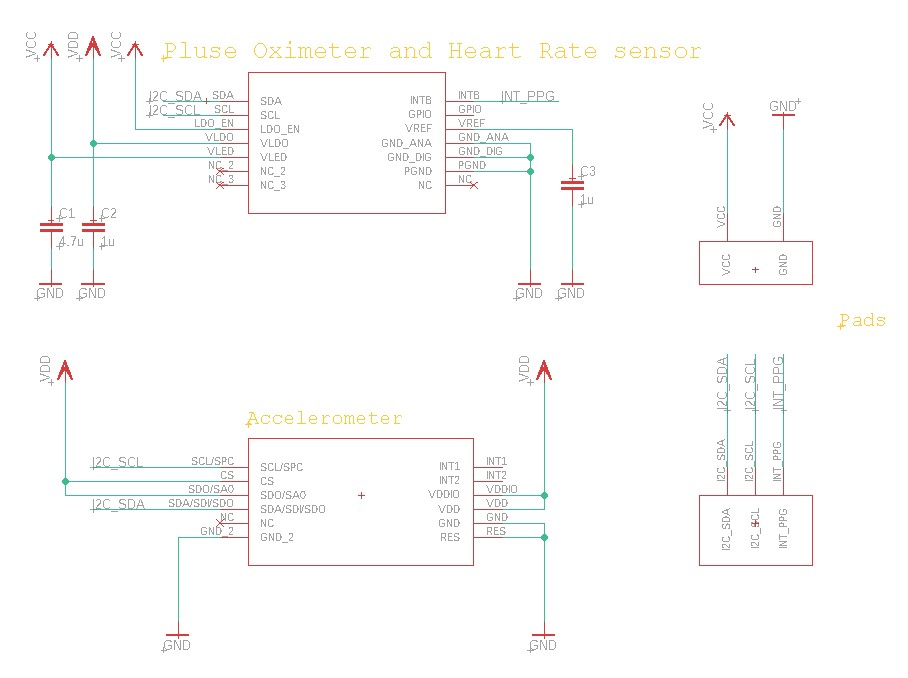
\includegraphics[width=0.8\linewidth]{ImageFiles/Hardware/schematic_maxm}
	\caption{Schematico Adapater Board con il sensore PPG MAXM86161}
	\label{fig:schematic_maxm}
\end{figure}
Il layout è stato prodotto partendo dallo schematico avendo cura di realizzare una board dalle dimensioni più ridotte possibili. Come si può vedere in figura \ref{fig:Layout_maxm} la board si compone su due layer, Top (in rosso) e Bottom (in blu).
\todo{Immagini da sistemare per metterle in fila a stessa dimensione}
\begin{figure}[h]
	\centering
	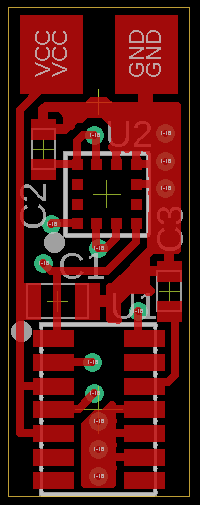
\includegraphics[width=0.15\linewidth]{ImageFiles/Hardware/layout_top_maxm}
	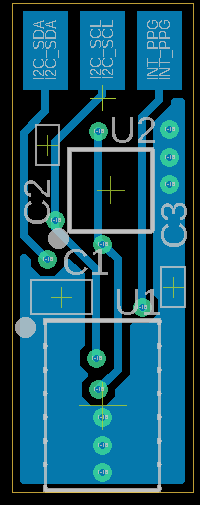
\includegraphics[width=0.15\linewidth]{ImageFiles/Hardware/layout_bottom_maxm}
	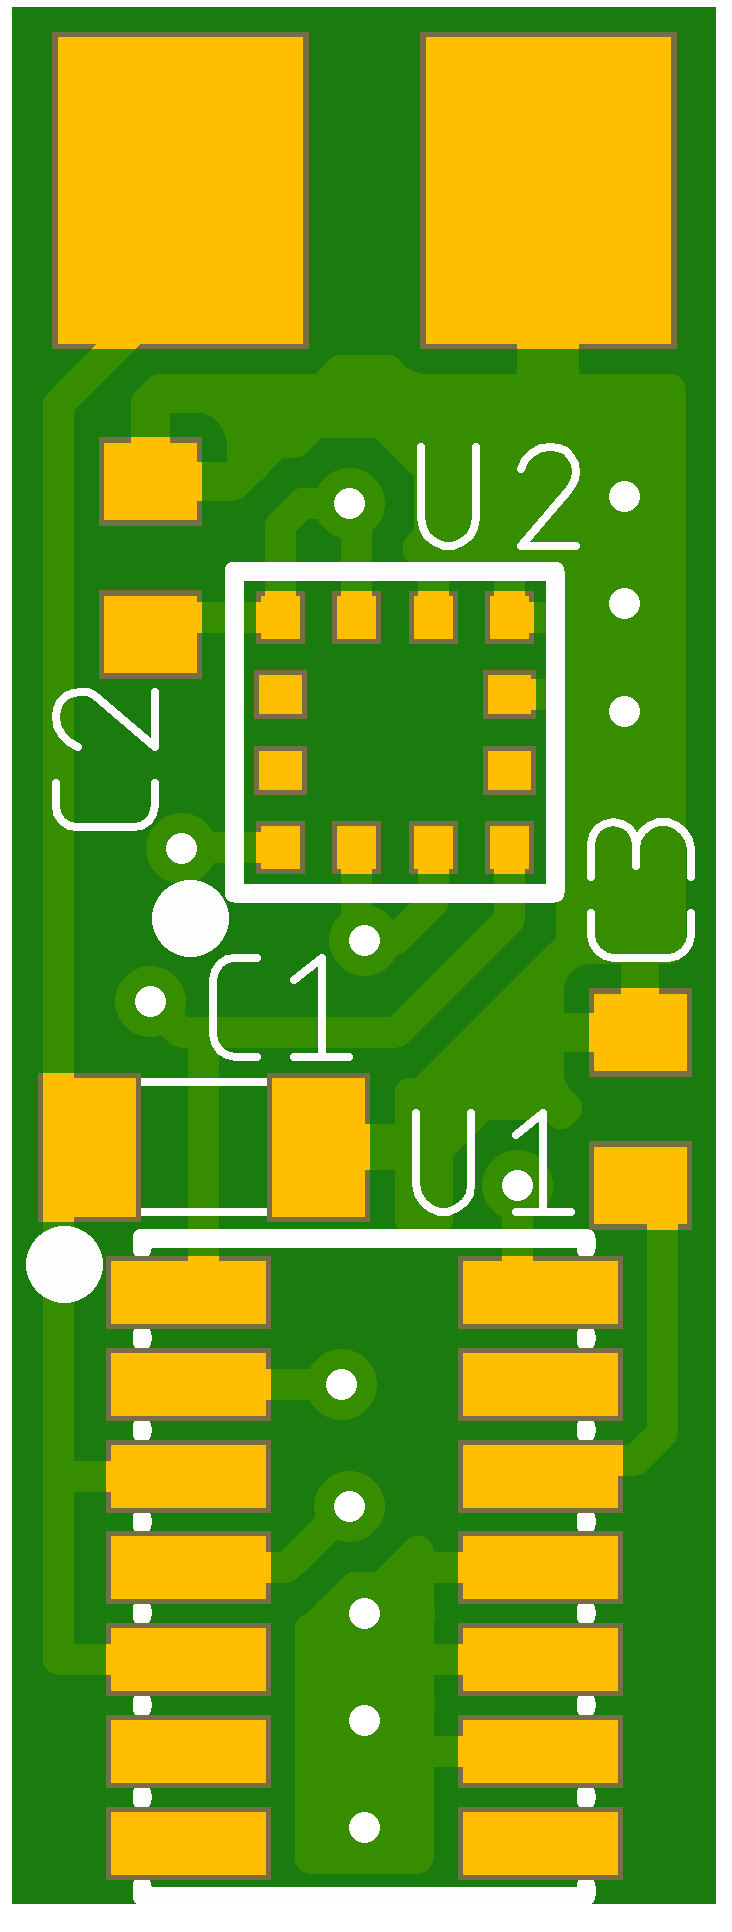
\includegraphics[width=0.15\linewidth]{ImageFiles/Hardware/manifacturing_top_maxm}
	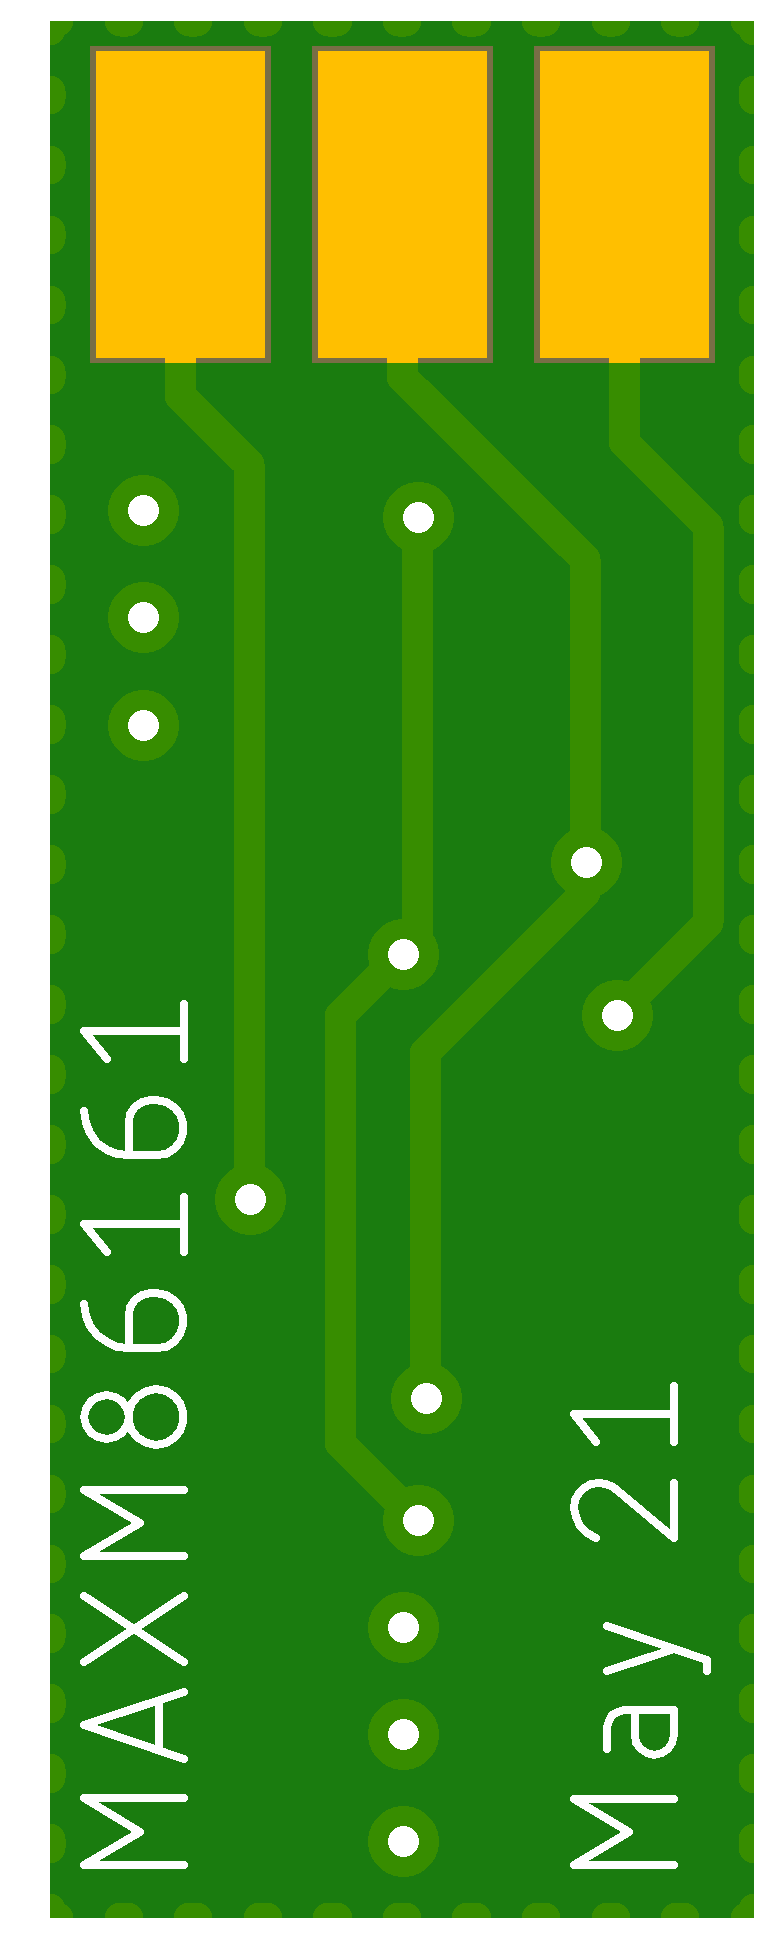
\includegraphics[width=0.15\linewidth]{ImageFiles/Hardware/manifacturing_bottom_maxm}
	\caption{Da sistemare}
	\label{fig:Layout_maxm}
\end{figure}
\subsection{Adapter Board: MAX86916}

\paragraph{Sensore PPG} Il sensore PPG utilizzato è il MAX86916, prodotto da Maxim Integrated, descritto precedentemente come stato dell'arte.

\begin{figure}[tb]
	\centering
	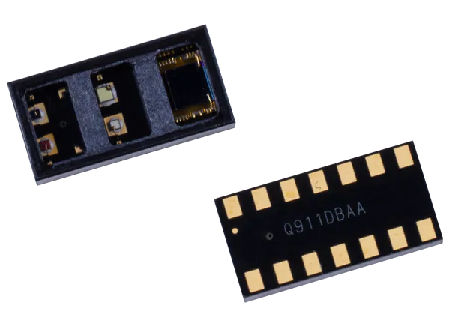
\includegraphics[width=0.6\linewidth]{ImageFiles/Hardware/ImmagineMAX86916}
	\caption{MAX86916 magari mettere in evidenza led e foto diodo}
	\label{fig:ImmagineMAX86916}
\end{figure}

\paragraph{LDO} \todo{Parliamo dei 3 LDO che abbiamo valutato? si parlerei di tutti e tre o almeno 2 mettendo in evidenza magari una tabella con le differenze}

\paragraph{Accelerometro}\todo{ut supra} L'accelerometro utilizzato è sempre \textbf{LIS2DH12} prodotto da STMicroelectronics.

\subsection{Microcontrollore: STM32F4DISCOVERY}\todo{farei una descrizione con alcune nozione sui componenti}
\todo{inserire immagine della board}